\documentclass[a4paper,DIV=17,dvipsnames,headsepline]{scrartcl}
\usepackage[utf8]{inputenc}
% \usepackage[margin=1in]{geometry}
\usepackage{graphicx}    % For including images
\usepackage{hyperref}    % For hyperlinks
\hypersetup{
    colorlinks=true,
    linkcolor=MidnightBlue,
    filecolor=magenta,      
    urlcolor=MidnightBlue,
    pdftitle={QuPath training},
    pdfpagemode=FullScreen,
    }
\usepackage{xcolor}      % For colored text (e.g., to highlight commands)
\usepackage{menukeys}   % forkeys and menu
\usepackage{listings}   % for code
\usepackage{siunitx}
\usepackage{lmodern}    % the font
\renewcommand{\familydefault}{\sfdefault}  % sans serif fonts
\usepackage{booktabs}   % nicer table
\usepackage{fourier}    % warning symbol
\pagestyle{headings}     % use srartcl headings style

\usepackage{enotez}      % create end notes with the solutions
\setenotez{backref=true}


\newcommand{\showsolutions}{\long\def\soln ##1\solnend{##1}}
\newcommand{\nosolutions}{\long\def\soln##1\solnend{}}

\showsolutions
%\nosolutions

\title{Nikon NIS-Elements\\ General Analysis 3}
\author{Dina Ratsimandresy, Jérôme Boulanger}
\date{May 2025}

\begin{document}

\maketitle

% \tableofcontents

\section{Introduction}

\subsection{Objectives}

\begin{itemize}
    \item Identify the image processing steps of a recipe such filtering, segmentation and binary processing.
    \item Manage records and table.
    \item Create a GA3 recipe for a given analysis problem.
    \item Batch process collection of files.
\end{itemize}

\subsection{General interface}

\paragraph{Preliminary steps}
Once the GA3 module opened, other windows cannot be opened, therefore
\begin{itemize}
    \item you will need to open the image you want to work with first,
    \item it is convenient to open the LUTs tools first (\keys{\ctrl+\Alt+L}).
\end{itemize}
To access the GA3 interface, you can either:
\begin{itemize}
    \item use the menu \menu{Image>New GA3 recipe\dots},
    \item use the menu \menu{Image>Analysis Explorer\dots} to open the analysis exporter and then click on \menu{Create New},
    \item right-click on the background of the interface, select \menu{Analysis Controls>Analysis Explorer} to open the analysis exporer and then click on \menu{Create New}.
\end{itemize}

\paragraph{Loading and saving recipes}

\begin{itemize}
    \item Use \menu{Save} or \menu{Save As} to save the recipe in the local database. It will be then listed in the Analyis Explorer.
    \item Use your name as a prefix so that we can contact you if the database needs to be cleared.
    \item Use \menu{Export} to export the recipe in a folder of your choice. This recipe can then be reloaded on another computer. It is good practice to have a copy of the recipes in that way.
    \item Use \menu{Import} to reload an exported recipe. 
\end{itemize}

\paragraph{Recipes}
\begin{figure}
    \centering \small
    \begin{tikzpicture}
        \node at (0,0) {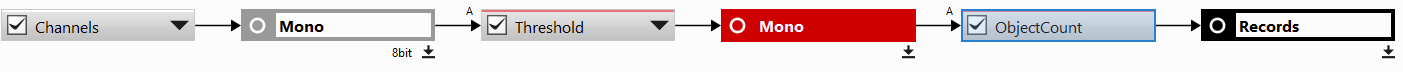
\includegraphics[width=0.75\textwidth]{artwork/simple-workflow.png}};
        % \draw[gray,very thin,step=1] (-5,-1) grid (5,1);
        \node (a) at (-5,-0.5){color};
        \node (b) at (-2,-0.5) {action};
        \node (c) at (0,-0.5) {binary};
        \node (d) at (4,-0.5) {table};
        \draw[->] (a) -| (-4,-0.2); 
        \draw[->] (b) -| (-1,-0.2); 
        \draw[->] (c) -| (1,-0.2); 
        \draw[->] (d) -| (5,-0.2); 
    \end{tikzpicture}
    \caption{A simple workflow with three kinds of nodes.}
    \label{fig:nodes}
\end{figure}

The recipes describes a workflow as a graph. The graph is compose of 4 types of nodes (See Fig.~\ref{fig:nodes}):
\begin{enumerate}\setlength\itemsep{0em}
    \item color: original or processed grayscale images
    \item action: processing steps on images, binary or tables
    \item binary: masks and labels
    \item results: tables with measurement results 
\end{enumerate}

To add an action, drag the new element to the previous one to automatically create a connection and keep the elements organized.

\paragraph{Storing results}

Saving of channels and binary layers can be enabled case by case using a right click on the layer. 

\subsection{Tips}
\begin{itemize}
    \item Use \keys{\Alt+\arrowkeyup} / \keys{\Alt+\arrowkeydown}  to increase / decrease the opacity of the binaries.
    \item To look for a module, use the search bar at the top.
    \item Right-click on the image and find image information for pixel to micron conversion.
    \item Click on the question mark on each operation (top left) for more information if needed.
\end{itemize}

\subsection{Image processing concepts}

\paragraph{Threshold}

\paragraph{Median filter} 

\paragraph{Rolling ball} Rolling ball is used for correcting shading and non-even background. It works by subtracting a background image estimated by dilating and eroding the image.

\paragraph{Watershed}



\subsection{Sample preparation and microscopy}

Lots of time can be saved by adjusting sample preparation and imaging to match existing  analysis tools.

\paragraph{Housekeeping labels} If possible, and when aiming at cell level statistics, include extra labels that will help identify cells location during sample preparation. A DNA stains such as DAPI and Hoescht and a plasma membrane marker such as WGA, Invitrogen's CellMask or Biotium's CellBrite can be used for example. 

\paragraph{Cell confluency} Depending on the type of analysis workflow and the cell line, high cell conflucency can be counterproductive as cell will tend to grow on top of each other.

\paragraph{Dataset size} When acquiring data, have in mind the scale of the process you want to capture. If only a fraction of the cells are of interest, define multiple position instead of tiling a large field of view at high resolution will reduce the size of the dataset.





 
\newpage
\section{Multi-image splitter}

\subsection{Problem}

Images of Invitrogen's FluoCell prepared slide with BPAE cells stained with MitoTracker Red CMXRos have been acquired on a Nikon ISIM microscope equipped with a multi image splitter. The software then always capture two images. However, only one marker was imaged and we would like to discard the blank image. We want to automatize this task to process several images at once and reduce the size of the dataset. The aim of this example is to illustrate the possibility to modify the original files using a GA3 recipe and potentially loose data.

\paragraph{Dataset} The three files \path{isim_001.nd2} .. \path{isim_003.nd2}  have two channels:
    \begin{enumerate}
        \item Red : Image from the frist camera to keep
        \item Blank : Image to discard
    \end{enumerate}

\paragraph{Concepts} Store results, Batch GA3


\subsection{Step-by-step instructions}
\begin{enumerate} 
    \item Open the image \path{isim_001.nd2} using \menu{File > Open} or a drag and drop.
    \item Open General Analysis 3 (see introduction)
    \item Select the Blank channel and select \menu{Do not Store this Result}. Note that a warning appear now at the bottom of the interface: ``Warning: Execution will remove some existing channels.''
    \item You can run the macro using \menu{Run now}, the image loaded in memory is modified, but the file is not saved.
    \item Save the recipe.
    \item Navigate to \menu{Image > Batch GA3}.
    \item Press the first icon \menu{Add files} and select the recipe and the three \path{isim_001.nd2} .. \path{isim_003.nd2}  files.
    \item Tick \menu{Keep Original} to save the results in a new set of files in a folder  \path{data/recipe_name +++BGM+++_date_time_}
    \item Press \menu{Run}.
    \item The jobs are now also listed under the recipe in the Analysis Explorer.
    \item Open the processed images from the folder \path{data/+++BGM+++_date_time_}
\end{enumerate}
\newpage
\section{Nuclei segmentation} \label{sec:nuclei-segmentation}

\subsection{Problem}

Segmenting the nuclei of cells in microscopy images is often the first step in the quantitative analysis of imaging data for biological and biomedical applications. Here we use an image of the Kaggle Science Data Bowl competition where cells were stained with DAPI or Hoechst. A basic approach based on classifying the pixels of a preprocessed image as foregroud and background using a threshold is used here.

\paragraph{Dataset} The file ``nuclei.tif'' has a single channel ``Mono''.

\paragraph{Concepts} preprocessing (Rolling Ball, Median), segmentation (Threshold), measurement (Circularity, Mean Obj Intensity, Object Area)


\paragraph{Reference} Caicedo, J.C., Goodman, A., Karhohs, K.W. et al. Nucleus segmentation across imaging experiments: the 2018 Data Science Bowl. Nat Methods 16, 1247–1253 (2019). \url{https://doi.org/10.1038/s41592-019-0612-7}

% 20 min

\subsection{Step-by-step instructions}
\begin{enumerate}
    \item Open the image ``nuclei.tif''.
    \item Start the GA3 module.
    \item Smooth the image using for example a median filter (\menu{Preprocessing > Median}) \endnote{radius:2px}.
    \item Correct uneven background using a rolling ball from \menu{Preprocessing > Rolling Ball} \endnote{radius:20px, signal is bright: ticked}.
    \item Classify the pixels of the image as foreground (nuclei) or background using a threshold. Drag the element \menu{Segmentation > Threshold > Threshold} on the previous step and adjust the parameters to segment the nuclei \endnote{Intensity range from 12 to 255, smooth:1x, clean:1x, fill holes:off, separate:2x, size:10-inf}.
    \item Measure the circularity and mean intensity of the segmented binaries using \menu{Measurement > Object shape > Circularity} and  \menu{Measurement > Object intensity > Mean Obj Intensity}\endnote{For measuring the mean intensity of objects, you'll need a binary mask (A) and an intensity mask (B).}. Dropping them on top of each other will automatically append the columns into a single table.
    \item To quickly inspect the properties of the measured regions, create a scatter plot using \menu{Results>Graphs>Scatterplot}.
\end{enumerate}


\newpage
\section{Synthetic cells}

\subsection{Problem}
In this problem, we make abstraction of the preprocessing steps and focus on the manipulation of binary layers. The image is a sketch representation of three cells with nuclei, cyctosol and some putative vesicles. We want to count the number of vesicle and the area of the nuclei area for each cell.

\begin{center}
\begin{tabular}{rrr}
    Cell ID& Number of endosomes& Nuclei area[px$^2$]\\
    1&8&6562\\
    2&13&7668\\
    3&9&11895\\
\end{tabular}   
\end{center}

\paragraph{Dataset:} The image is \path{synthetic_cells.nd2} with the following channels:
\begin{itemize}\setlength\itemsep{0em}
    \item red: endosomes
    \item green: cytoplasm
    \item blue: nuclei
\end{itemize}

\paragraph{Concepts} object parenting (ParentID, Child ID, Aggregate Children), data management (GroupRecords, AggegateRows, ModifyColumns, JoinRecords, Aggregate Children), measurement (ObjectArea)

\begin{description}
    \item[Task:] For each cell, count the number of red dots and measure the area of the nuclei.
    \item[Data:] ``synthetic cells.nd2'' with three channels: dots (red), cytoplasm (green) and nuclei (blue). 
    \item[Topics:] object parenting (ParentID, Child ID, Aggregate Children), data management (GroupRecords, AggegateRows, ModifyColumns, JoinRecords, Aggregate Children), measurement (ObjectArea)
    \item[Duration:] 30 min
    \item[Step by step:]
\end{description}

\subsection{Step-by-step instructions}

\begin{enumerate}
    \item Load the image ``synthetic cells.nd2''.

    \item Create binary masks for all the channels with the names ``endosomes'', ``cells'' and ``nuclei'' \endnote{Use a threshold with value 128-255 for example.}. 

    \item For creating a parent-child hierarchy associating the endosomes to the cells and count the number of endosomes per cell, add the action \menu{Measurement>Object parenting>Aggregate Children} with A (parent): ``cells'' binary and B (child): ``endosomes''. 

    % \begin{description}
    %     \item[Option 1] Associate a parent to each endosome and group the records
    %     \begin{itemize}
    %         \item To associate a cell to each dot,  use \menu{Measurement > Object parenting > Parent ID} linking A (parent) to the ``cytoplasm'' binary and B (child) to the ``dots'' binary.
    %         \item Group the row by adding a module \menu{Data Management > Grouping > Group Records} and use cytoplasmID.    
    %         \item Add the module \menu{Data Management > Grouping >  Aggregate Rows} and set the line ``ObjectId'' to ``Count'' in AggregateRows. 
    %     \end{itemize}

    %     \item[Option 2] Associate a list of child to each cytoplasm and group the records
    %     \begin{itemize}
    %     \item Associate for each cytoplasm, the list of endosomes using \menu{Measurement > Object parenting > Child ID} linking A (parent) to the ``cytoplasm'' binary and B (child) to the ``endosomes'' binary.
    %     \item Group the row by ObjectId using the action \menu{Data Management > Grouping > Group Records} 
    %     \item Add the action \menu{Data Management > Grouping > Aggregate Rows} and set ``dotsID'' to ``Count'' 
    %     \end{itemize}

    %     \item[Option 3] The element ``Aggregate children'' enable to compute parenting and aggregate by parent at once.
    %     \begin{itemize}
    %         \item Drop the module \menu{Measurement>Object parenting>Aggregate Children} on the ``cytoplasm'' binary and link B (child) to the ``endosomes'' binary. 
    %     \end{itemize}
    % \end{description}

    \item Measure the area of each nuclei using \menu{Measurement > Object Size > Object Area}.
    
    \item Add the cell ID to the records of nuclei area using \menu{Measurement > Object parenting > Parent Id} with A (parent) to the ``cell'' and B (child) to the ``nuclei'' binary. 
    
    \item Use \menu{Data Management > Basic > Join Records} to join using ``Object Id'' for tables A and B linking the area measurements and the parenting.
    
    \item Group the row by ``CellId'' using the action \menu{Data Management > Grouping > Group Records} 
    
    \item Add the action \menu{Data Management > Grouping > Aggregate Rows} and set ``Object Area'' to ``Sum'' 
    
    \item Use \menu{Data Management > Basic > Join Records} to join using ``Cell Id'' for tables A and B.
    
    \item Use \menu{Data Management > Basic > Rename Columns} to keep only the necessary columns.

\end{enumerate}

% \newpage
% \section{Selective cargo tethering}

\subsection{Problem}

In this example, we are interested into quantifying the capture of syntaxin-16 cargos vesicles by the mitochondria when the protein TBC1D23 is relocated to the mitochondria. We want to quantify for each cell the level of colocalization between the mitochondria and the cargo to measure the effect of mutant of TBC1D23 on the effectivness of the cargo tethering. Note that not all cells are transfected.


\paragraph{Dataset} Prepared cells were imaged using a Zeiss confocal microscope using a 63x/1.4NA oil immersion lens. We will use the file ``Zeiss1344.lsm'' which have the following channels:

\begin{itemize}\setlength\itemsep{0em}
    \item Ch2-T1 : Golgi maker GM130
    \item ChS2-T2 : cargo protein
    \item ChS1-T3 : mitochondria
    \item Ch1-T4 : nuclei marked with DAPI
\end{itemize}

\paragraph{Concepts} Segmentation with seeded watershed (Threshold, DistanceFunction, Watershed, GrowObjects), colocalization (Pearson Coeff), data management (AppendColumns, Binning, GroupRecords, AppendColumns), display (Barchart).

\paragraph{Credit}  Alison Gillingham from Sean Munro's group at the MRC-LMB

\paragraph{Reference} Jérôme Cattin-Ortolá et al., Cargo selective vesicle tethering: The structural basis for binding of specific cargo proteins by the Golgi tether component TBC1D23. Sci. adv.10,eadl0608(2024). 

DOI:10.1126/sciadv.adl0608

\subsection{Step-by-step instructions}
\begin{enumerate}
    \item Open the image ``Zeiss1344.lsm''. A windows pop up asking if the image is part of a sequence. Click on the \menu{Leave} button.
    \item Segment the cells using a seeded watershed approach by following the three steps below:
    \begin{enumerate}
        \item Create a mask for the cells using the Golgi marker (Ch2-T1) channel using \menu{Preprocessing > Convolution > Gaussian Filter} and \menu{Segmentation>Threshold} \endnote{filter radius:2px, threshold 1-255, smooth:, clear:}. Note that the image bit depth changed to 32-bit after filtering.
        \item Segment the nuclei using \menu{Segmentation>Threshold} \endnote{threshold: 30-inf, smooth \SI{1}{\micro\meter}, clean , \SI{1}{\micro\meter}, fill holes OFF, Separate OFF and size \SI{5}{\micro\meter}-1000.}.
        \item Add the action \menu{Binary processing > Detect > Distance function} to the Golgi marker (Ch2-T1) binary. 
        \item Use the \menu{Binary processing> Region growing > Watershed} select the type ``From Bright Regions''. 
        \item Use \menu{Binary operations > And} linking the result of the watershed (Ch1-T4) and the initial cell mask (Ch2-T1) to restrict the mask to the cells.
        \item Rename the binary as ``Cells''.
    \end{enumerate}
    \item Use \menu{Measurement > Object ratiometry > Pearson Coeff} to measure the colocalization coefficient between the Golgi (Ch2-T1, link to B) and cargo protein (ChS2-T2, link to C) within the segmented region (binary to link to A). 
    \item Repeat to measure the colocalization coefficient between the mitochondria and cargo protein.
    \item Measure the mean intensity of the mitochondria channel using \menu{Measurement > Object Intensity > Mean}.
    \item Merge the three records table together using \menu{Data Management > Basic > AppendColumns}.
    \item At this point make sure that the workflow doesn't remove any channel
    \item Save the recipe
    \item Export all images lsm as nd2 files using \menu{File>Import/Export>Convert files}.
    \item Open the batch processing module using \menu{Image>Batch GA3}.
\end{enumerate}

% \newpage
% \section{Particle tracking}

\begin{description}
    \item[Task:] Track simulated single particle moving in the field of view.
    \item[Data:] ``synthetic beads.nd2'' with one channel and 20 time points.
    \item[Topics:] Segmentation (Bright Spots), Tracking (Time \& centroid, Track Particles, Accumulate \& group, Speed), Measurement (Mean Obj Intensity), Results (Linechart)
    \item[Duration:] 40 min
    \item[Step by step:]
\end{description}

\begin{enumerate}
    \item Open the file ``synthetic beads.nd2'' and create a new General Analysis 3 workflow.
    \item Detect the particles in the image. \soln Use \menu{Segmentation>Spot Detections>Bright Spots} with diameter 0.5 and contrast 2. \solnend
    \item Extract the centroid of each particle. \soln Use the \menu{Tracking>2D Object Position>Time \& Centroid}. \solnend
    \item Measure the mean intensity of each particle. \soln Use \menu{Measurement>Object intensity>Mean Obj Intensity}. \solnend
    \item Merge the two tables to have the centroid and the mean intensity of each particle in one table.  \soln Use \menu{Data Management>Basic>Join Records} using the ObjectId to link the tables A and B. \solnend
    \item Track the particles over time. Use \menu{Tracking > 2D Tracking > Track Particles} with ``Time Column'' set to "TimeLapseIndex" or "Time"\soln and ``Maximum Speed'' set to 5 \solnend. Add \menu{Tracking > Tracks > Accumulate \& Group}. Tracking objects applies to the image while track particle applies to the records; max speed corresponds to max speed of the objects between consecutive frames (however not working in the software at the moment), while max gap size is max allowed skipped frames.
    \item Measure the speed of each tracked particle. \soln Use \menu{Tracking > Tracking features > Speed} and set ``DiffTime'' to Time. \solnend
    \item Display the tracks. Use \menu{Results > Linechart}, in the Data tab use ``CentroidX'' for theh ``X Axis'' and ``CentroidY'' for the ``Y Axis Left''.
\end{enumerate}

\begin{description}
    \item[Optional:] Use the tracking module on the binaries generate by the workflow.
\end{description}

% \newpage
% \pagebreak
\nsection{Infected cells}

\begin{description}
    \item[\entry{Task:}] Evaluate the number of infected cells by the number of bacteria detected in each of the cells. 
    \item[\entry{Data:}] ``Infected cells.nd2'' with four channels: nuclei marked by DAPI (blue), bac1 (green), bac2 (red), bac3 (cyan).\textcolor{olive}{I noticed there is a bac3 copy channel in the data now.}
    \item[\entry{Topics:}] Preprocessing (Gaussian filters), Segmentation (Bright Spots), Binary processing (Grow regions), Data management (Aggregate Children, Append Columns).
    \item[\entry{Acknowledgement:}] Agnes Foeglein
    \item[\entry{Duration:}] 40 min
    \item[\entry{Step by step:}]
\end{description}

\begin{enumerate}
    \item Open the file “Infected cells.nd2” and start General Analysis 3
    \item Segment the cells using the DAPI channel. \soln Use \menu{Preprocessing>Gaussian filters} with filter “Gaussian” and “sigma” 10. Use \menu{Segmentation>Spot Detections>Bright Spot} with diameter 10, contrast 20, symmetry all, Intensity above “30”. Add \menu{Binary Processing>Region growing>Grow Regions} linking A to the binary and B to the filtered image. \solnend
    \item Segment the bacteria in channels bac1, bac2, bac3. \soln Use \menu{Segmentation > Spot Detections > Bright Spot} with diameter \SI{1}{\micro\meter}, contrast 20, intensity above 150. \solnend
    \item For each cell, count the number of each type of bacteria. \soln Use \menu{Measurement > Object parenting > Aggregate Children} three times with the DAPI binaries as parent and each bac1, bac2, bac3 binaries as children. Merge the 3 tables into one using \menu{Data Management>Basic>Append Columns}. \solnend
\end{enumerate}

% \newpage
% \section{Cell division in dendraster excentricus}

\begin{description}
    \item[Task:] Track the cells along the division and count the number of cells over time.
    \item[Data:] ``cell division.tif'' with one channel and 200 time points.
    \item[Topics:] preprocessing (Rolling Ball), segmentation (Threshold), object tracking, measurement (Object Count), results (Linechart)
    \item[Reference:] 
        George Von Dassow (2011) CIL:15798, Dendraster excentricus. \\
        CIL.Dataset. https://doi.org/doi:10.7295/W9CIL15798
    \item[Duration:] 40 min
    \item[Step by step:]
\end{description}

\begin{enumerate}
    \item Open the image ``cell division.tif'' and create a new GA3 workflow.
    \item Segment the nuclei of each cell. \soln Use \menu{Preprocessing>Background>Rolling Ball} with a radius of 10px followed by \menu{Segmentation>Threshold>Threshold} with intensity above 10, Smooth 8x, Clean 1x, FillHoles OFF, Separate 1x and Size[px] above 5px. \solnend
    \item Make sure that the Binaries are stored but that channels are not modified.
    \item Count the number of cell for each time point. Use \menu{Measurement>Whole Field>Object Count} and \menu{Tracking>Tracks>Accumulate \& Group}.
    I would put these two operations into two separate point; keeping the object count as it is and add the following point for tracking
    \item Track the cells over time. Use \menu{Tracking > 2D Tracking > Track Particles} with ``Time Column'' set to "TimeLapseIndex" or "Time"\soln and ``Maximum Speed'' set to INF \solnend. Add \menu{Tracking > Tracks > Accumulate \& Group}.
    \item Graph the number of cells over time. Use \menu{Results>Graphs>Linechart}
    \item Run the recipe on all frames. 
    \item Use the tracking app from the main interface to track all the binaries.
    Click on tracking options; allow track split; observe from the image stack and estimate how many mitosis happen on average over the time period and determine probability.
\end{enumerate}


\appendix
\printendnotes

\end{document}
